% !TEX root = ../Coherence2.tex

\section{Contextual nestohedra} 
\label{s:contextual}

We define special families of hypergraph polytopes (nestohedra) which we call ``contextual'', and exhibit several examples.
As we will see in the next sections, these families have associated term rewriting systems, and in some cases exhibit coherence for categorified algebraic structures.

%%%%%%%%%%%%%%%%%%%%%%%%%%%%%%%%%%%%%%%

\subsection{Definition}

\begin{definition}
  A connected hypergraph $\hyper{H}$ is \defn{contextual} if for all connected subsets $Y \subseteq H$ of cardinal $|Y|\geq 3$, and for all subsets $X \subseteq Y$ of cardinal $|X|=3$, we have
  $$\hyper{H}_{\cap X} = (\hyper{H}_Y)_{\cap X}.$$ 
\end{definition}

\begin{lemma} \label{context-lemma}
A connected hypergraph $\hyper{H}$ is contextual if for all connected subsets $Y\inc H$ of cardinal $|Y|\geq 3$, and for all $3$-elements subsets $X=\{x,y,z\} \subseteq Y$, we have 
$$\begin{array}{lll}
  \xyz{x}{{\hyper{H}_Y}}{\set{y,z}} & \Leftrightarrow & \xyz{x}{\hyper{H}}{\set{y,z}}.
  \end{array}$$
\end{lemma}
 
\begin{proof} 
  This is a direct consequence of Lemma~\ref{xyz-reconnected}.
\end{proof}

For a 3-element subset $X=\set{x,y,z}$ of $H$, we say that a 2-face of $\hyper{H}$ is an \defn{$X$-face} if its unique non-singleton node is decorated by $X$.

\begin{example} \label{non-contextual-1}
Consider the hypergraph 
$$\hyper{H}= \set{\set{x},\set{y},\set{z},\set{u},\set{x,y,z}, \set{x,u,z}}$$
and its two $\set{x,y,z}$-faces $S=u(\set{x,y,z})$ and $T=\set{x,y,z}(u)$. 
Then $\occ{S}{\set{x,y,z}}$ is a construct of
$\hyper{K}=\restrH{H}{\set{u}}$ while $\occ{T}{\set{x,y,z}}=T$ is a construct of $\hyper{H}$.
But we have $\xyz{y}{\hyper{K}}{\set{x}\!,\!\set{z}}$ while  $\xyz{y}{\hyper{H}}{\set{x,z}}$. 
As a matter of fact,
$S$ is a triangle while $T$ is a quadrilateral, since
$$\begin{array}{lllll}
\recrestr{\hyper{K}}{\set{x,y,z}} &=& \hyper{K} & = & \set{\set{x},\set{y},\set{z},\set{x,y,z}}\\
\recrestr{\hyper{H}}{\set{x,y,z}} && =&&  \set{\set{x},\set{y},\set{z},\set{u},\set{x,z}\set{x,y,z}}.
\end{array}$$
\end{example}
  
\begin{example} \label{non-contextual-2}
Consider the graph 
$$\set{\set{x},\set{y},\set{z},\set{u},\set{x,y}, \set{y,z}, \set{x,u}, \set{u,z}}$$
Then exactly the same data as in Example \ref{non-contextual-1} provide evidence that this graph, whose realisation is the three-dimensional cyclohedron, is not contextual. 
\end{example}

The definition of contextual hypergraph was motivated by the following observation: if $X$ is the root of $T$, one can see $T=X(\ldots)$ as an ``instantiation'' of $X$, viewed as the maximum face of $\recrestr{\hyper{H}}{X}$.

\begin{lemma} \label{instance-construct} 
 If $\hyper{H}$ is a connected hypergraph, if $X$ is a subset of $H$ such that $|X|=3$ and $T$ is a 2-dimensional construct with root $X$, then the poset of faces of $T$ is isomorphic to the poset of faces of $\recrestr{\hyper{H}}{X}$.
\end{lemma}

\begin{proof}
In Section~\ref{s:anatomy}, we have described (cases (a), (b), (c) and (d)) up to permutation all the possible connected hypergraphs on the set $\set{x_1,x_2,x_3}$ of vertices and their respective posets of faces. Suppose, say, that
 ${\cal A}(\recrestr{\hyper{H}}{X})$ is the poset underlying the picture of case (B.c). Pick, say the 0-face $S= x_1(x_2,x_3)$. We map $S$ to a 0-subface $\phi(S)$ of $T$ as follows. Let $\hyper{H},\set{x}\leadsto H_1,\ldots,H_n$. By Lemma \ref{xyz-reconnected}, we have $\xyz{x_1}{\hyper{H}}{\set{x_2},\set{x_3}}$, hence we have, say $x_2\in H_1$ and $x_3\in H_2$. Then let
 $\hyper{H_1},\set{x_2}\leadsto H_{1,1},\ldots,H_{1,p}$ and $\hyper{H_2},\set{x_3}\leadsto H_{2,1},\ldots,H_{2,q}$.
 Then we have $\hyper{H},X\leadsto H_{1,1},\ldots,H_{1,p},H_{2,1},\ldots,H_{2,q},H_3,\ldots H_n$, so that $T$ writes as
 $T= X(T_{1,1},\ldots,T_{1,p},T_{2,1},\ldots,T_{2,q},T_3,\ldots T_n)$. All these data determine uniquely a 0-dimensional subface of $T$, namely
 $$\phi(S)=x_1(x_2(T_{1,1},\ldots,T_{1,p}),x_3(T_{2,1},\ldots,T_{2,q}),T_3,\ldots T_n)$$
and one recovers $S$
 by  pruning in $\phi(S)$ all nodes except those decorated by subsets of $X$.
 The same applies to all other 0-dimensional (resp. 1-dimensional) faces of $\recrestr{\hyper{H}}{X}$, establishing $\phi$ as a bijection, which is also easily seen to be monotonic: for example, we have
$$\phi(\set{x_1,x_2}(x_3))= \set{x_1,x_2}(x_3(T_{2,1},\ldots,T_{2,q}),T_{1,1},\ldots,T_{1,p},T_3,\ldots T_n),$$
evidencing $\phi(x_1(x_2,x_3))\preceq \phi(\set{x_1,x_2}(x_3))$. 
The inverse of $\phi$ is also monotonic, since the above pruning does not affect the place where the contraction occurs -- e.g., the edge of $\phi(x_1(x_2,x_3))$ that is contracted to get $\phi(\set{x_1,x_2}(x_3))$ is the edge between $x_1$ and $x_2$, which can thus be contracted in the preimage $x_1(x_2,x_3)$ to yield the preimage $\set{x_1,x_2}(x_3)$.
Finally, we set
$$\phi(\set{x_1,x_2,x_3})=\set{x_1,x_2,x_3}(T_{1,1},\ldots,T_{1,p},T_{2,1},\ldots,T_{2,q},T_3,\ldots T_n)=T.$$
\end{proof}

Now, if $T'$ is another $X$-face and $\occ{T'}{X}\neq T'$ (i.e., $X$ is not the root of $T'$), then we would like to see  $T'$ as $\occ{T'}{X}$ in context, and hence $T'$ as ``$X$ in situation''.  
This can be done precisely when $\hyper{H}$ is contextual.


%But, to be able to see $X$ as a ``coherence condition'', we should have that all $X$-faces have isomorphic posets of faces.  
%Is it the case?  
%Let us take $T,T'$ as  above: the poset of subfaces of $T'$ is isomorphic to the poset of subfaces of $\occ{T'}{X}$, which is a construct of $\hyper{H}_E$, where $E={supp}(\occ{T}{X})$ and has $X$ as root, so that the latter poset (and hence the former) is isomorphic to the poset of faces of $\recrestr{\hyper{(H_E)}}{X}$.
%Is it always the case that $\recrestr{\hyper{(H_E})}{X}=\recrestr{\hyper{H}}{X}$ for $E$ connected in $\hyper{H}$? The following examples give a negative answer.

\begin{proposition} \label{situation-construct}
Let $\hyper{H}$ be a contextual hypergraph.
If $X$ is a subset of $H$ such that $|X|=3$ and $T$ is an $X$-face of $\hyper{H}$, then the poset of faces of $T$ is isomorphic to the poset of faces of $\recrestr{\hyper{H}}{X}$.
\end{proposition}

\begin{proof} 
  Let $\hyper{K}=\hyper{H}_{\supp(S)}$ where $S=\occ{T}{X}$. 
  By \cref{subconstruct-restriction}, $S$ is a constuct of $\hyper{K}$. By definition of the face relation, and since the only non-singleton (and hence ``splittable'') node of $T$ is $X$, we have that the poset of subfaces of $T$ is isomorphic to the poset of subfaces of $S$, which by \Cref{instance-construct} is isomorphic to ${\cal A}(\recrestr{\hyper{K}}{X})$, which is isomorphic to ${\cal A}(\recrestr{\hyper{H}}{X})$ since $\hyper{H}$ is contextual.
\end{proof}

Proposition~\ref{situation-construct} allows us to see all $X$-faces as ``instantiations in context'' of $\recrestr{\hyper{H}}{X}$, which therefore acts  as a rule or axiom in the terminology of equational theories.
Motivated by the examples presented below in \cref{ss:examples} and their associated categorical coherence theorems, we define now the notion of a contextual \emph{family} of nestohedra.

Formally, the following proposition says that, if $\hyper{H}$ is contextual, any such local confluence diagram, stemming from any $\set{x_1,x_2,x_3}$-face, is an instance in context of a local confluence diagram in $\recrestr{\hyper{H}}{\set{x_1,x_2,x_3}}$ (which depends only on $\hyper{H}$ and ${x_1,x_2,x_3}$) and hence is determined by the latter, which therefore deserves the name of coherence condition

\begin{proposition} Given a contextual hypergraph $\hyper{H}$ and a total order on $H$, all order-isomorphisms
of
Proposition \ref{situation-construct} preserve and reflect the flip order on constructions, i.e.  $S$ rewrites to $S'$ according to this order if and only if the image of $S$ rewrites to the image of $S'$.
\end{proposition}

\begin{proof} The proof is an easy variation on the proof of Lemma~\ref{instance-construct}. 
\end{proof}

Identifying an hypergraph $\hyper{H}$ with the maximal construct $T$ of $({\cal A}(\hyper{H}),\preceq)$, we say that $\hyper{H}$ has \defn{dimension} $\dim T$.

\begin{definition}
    A family $\calH=\{\calH(n)\}_{n\geq 0}$ of hypergraphs is \defn{contextual} if 
    \begin{enumerate}
      \item any hypergraph $\hyper{H} \in \calH$ is contextual,
      \item every $2$-dimensional hypergraph in $\calH(2)$ is isomorphic to $\hyper{H}_{\cap X}$ for some $X$-face of an hypergraph $\hyper{H} \in \calH(n)$ with $n\geq 3$. 
    \end{enumerate}
\end{definition}

%%%%%%%%%%%%%%%%%%%%%%%%%%%%%%%%%%%%%%%

\subsection{Examples}
\label{ss:examples}

Let us briefly introduce some families of hypergraph polytopes, that will be shown in \cref{thm:examples} to be contextual. 
Recall that any graph can by considered an hypergraph with no hyperedges.
The resulting hypergraph polytopes are known as \emph{graph-associahedra} \cite{CD-CCGA}.

\subsubsection{Simplices}
The $n$-dimensional \defn{simplex} is the realization of the hypergraph 
$$\mathbb{S}_n:=\{\{x_1\},\{x_2\},\ldots,\{x_{n+1}\},\{x_1,\ldots,x_{n+1}\}\}.$$

\subsubsection{Cubes}
The $n$-dimensional \defn{cube} is the realization of the hypergraph
$$\mathbb{C}_n:=\{\{x_j \ | \ 1 \leq j \leq i \} \ | \ 1 \leq i \leq n+1\}.$$

\begin{rem}
  Note that these two families of hypergraph polytopes are defined by genuine hypergraphs, contrary to the following families of graph-associahedra.
\end{rem}

\subsubsection{Associahedra}
The $n$-dimensional \defn{associahedron} is the realization of the hypergraph 
$$\mathbb{K}_n:=\{\{x_1\},\{x_2\},\ldots,\{x_{n+1}\},\{x_1,x_2\},\ldots,\{x_n,x_{n+1}\}\}.$$
In other words, it is the graph-associahedron for the linear graph with $n+1$ vertices.

\subsubsection{Permutahedra}
The $n$-dimensional \defn{permutahedron} is the realization of the hypergraph 
$$\mathbb{P}_n:=\{\{x_1\},\{x_2\},\ldots,\{x_{n+1}\}\} \cup \{\{x_i,x_j\} \ | \ 1 \leq i \neq j \leq n+1 \}.$$
In other words, it is the graph-associahedron for the complete graph on $n+1$ vertices.

\subsubsection{Operahedra}
To every rooted planar tree $\calT$ with $n+2$ vertices, one can associate its $n$-dimensional \defn{operahedron}, whose faces are in bijection with nestings of $\calT$ \cite{laplante-anfossiDiagonalOperahedra2022a,CLA1}.
These are in bijections with the tubings of the \defn{line graph} $\mathbb{L}(\calT)$ of $\calT$.
The vertices of $\mathbb{L}(\calT)$ are the edges of ${\cal T}\!$, and two vertices are connected whenever as edges of ${\cal T}$ they share a common vertex, see \cref{fig:line-graph}.
In other words, an $n$-dimensional operahedron is the graph-associahedron for a clawfree block graph with $n+1$ vertices.

\begin{figure}[h!]
  \begin{center}
    \begin{tabular}{ccc}
    \resizebox{2cm}{!}{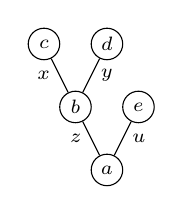
\begin{tikzpicture}[scale=0.8]
        % set up the nodes
        \node (E)[circle,draw=black,minimum size=4mm,inner sep=0.1mm] at (0,0) {\scriptsize $a$};
        \node (F) [circle,draw=black,minimum size=4mm,inner sep=0.1mm] at (-0.5,1) { \scriptsize $b$};
        \node (A) [circle,draw=black,minimum size=4mm,inner sep=0.1mm] at (0.5,1) {\scriptsize $e$};
        \node (Asubt) [circle,draw=black,minimum size=4mm,inner sep=0.1mm] at (-1,2) {\scriptsize  $c$};
        \node (P) [circle,draw=black,minimum size=4mm,inner sep=0.1mm] at (0,2) {\scriptsize $d$};
        % draw arrows and text between them
        \draw[-] (E)--(F) node  [midway,left] {\scriptsize $z$};
        \draw[-] (E)--(A) node  [midway,right] {\scriptsize $u$};
     \draw[-] (F)--(Asubt) node [midway,left] {\scriptsize $x$};
     \draw[-] (F)--(P) node [midway,right] {\scriptsize $y$};
       \end{tikzpicture}}
    
    &&
    \resizebox{2cm}{!}{
    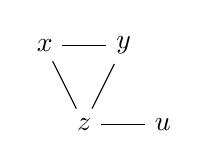
\begin{tikzpicture}
        % set up the nodes
        \node (Z)[] at (-0.5,0) {$z$};
        \node (U)[]  at (0.5,0) {$u$};
        \node (X)[]  at (-1,1) {$x$};
        \node (Y)[]  at (0,1) {$y$};
        % draw arrows and text between them
        \draw[-] (Z)--(U) node  {};
     \draw[-] (Z)--(X) node  {};
     \draw[-] (Z)--(Y) node {};
     \draw[-] (X)--(Y) node {};
       \end{tikzpicture}}
    \end{tabular}
    \end{center}
    \caption{A planar tree with $5$ vertices (left) and its line graph (right).}
    \label{fig:line-graph}
\end{figure}

\subsubsection{Contextual graph-associahedra}
We call \defn{contextual graph-associahedra} the hypergraph polytopes whose underlying hypergraph is a connected simple graph which is moreover contextual.
This family includes all the three previous families, but is far from containing all graph-associahedra.
For instance, we have seen in \cref{non-contextual-2} that the well-known cyclohedra are \emph{not} part of this family. 

\subsubsection{Contextual nestohedra}
We call \defn{contextual nestohedra} the family of hypergraph polytopes whose underlying hypergraph is contextual. 

\begin{rem}
  It would be interesting to characterize combinatorially contextual graphs and hypergraphs.
\end{rem}



\begin{thm}
  \label{thm:examples}
  The following families of hypergraph polytopes are contextual:
  \begin{enumerate}
    \item simplices,
    \item cubes,
    \item associahedra,
    \item permutahedra,
    \item operahedra,
    \item contextual graph-associahedra,
    \item contextual nestohedra.
  \end{enumerate}
\end{thm}

\begin{proof}
  Let us proceed one family at a time.
  \begin{enumerate}
    \item simplices,
    \item We first note that the above description of $\hyper{C}_n$ is saturated, and that $(\hyper{C}_n)_{\set{1,\ldots,m}}=\hyper{C}_m$ (if $m\leq n$).
    So we have to check that  for all $m\leq n$ and all $i,j,k\leq m$, we have $\xyz{k}{{\hyper{H}_n}}{\set{i,j}}$ iff
    $\xyz{k}{{\hyper{H}_m}}{\set{i,j}}$, which follows immediately from the observation that for all $p\geq m$ we have
    $\xyz{k}{{\hyper{H}_p}}{\set{i,j}}$ iff $i<k$ and $j<k$.
    \item associahedra,
    \item permutahedra,
    \item It is proved in~\cite[Lem.~12]{COI} that the connected subsets of $\hyper{G}({\cal T})$ are in bijective correspondence with the subtrees of $\cal T$ having at least two nodes, through a map $E\mapsto  {\cal T}_E$ such that $\hyper{G}({\cal T})_E=\hyper{G}({\cal T_E})$. Suppose, say, that $\set{x,y,z}\inc E$ and $\xyz{x}{\hyper{G}({\cal T})_E}{\set{y},\set{z}}$. Then it means on the tree side that after removing the edge $x$ from ${\cal T}_E$, resulting in two disjoint subtrees ${\cal T}_E^1$ and ${\cal T}_E^2$ of ${\cal T}_E$, we have, say, $y\in{\cal T}_E^1$ and $z\in{\cal T}_E^2$. 
    On the other hand, removing $x$ from ${\cal T}$ results in subtrees ${\cal T}^1$ and ${\cal T}^2$, containing ${\cal T}_E^1$ and ${\cal T}_E^2$, respectively. 
    Therefore $\xyz{x}{\hyper{G}({\cal T}))}{\set{y},\set{z}}$. 
    And vice-versa.
    \item We only need to check that every $2$-dimensional contextual graph-associahedron appears as a $2$-face of a higher dimensional contextual graph-associahedron. 
    \item We only need to check that every $2$-dimensional contextual nestohedron appears as a $2$-face of a higher dimensional contextual nestohedron.
  \end{enumerate}
\end{proof}









